\section{MOTIVATING EXAMPLE}
\label{sec:mot}

\begin{figure}
	\centering
	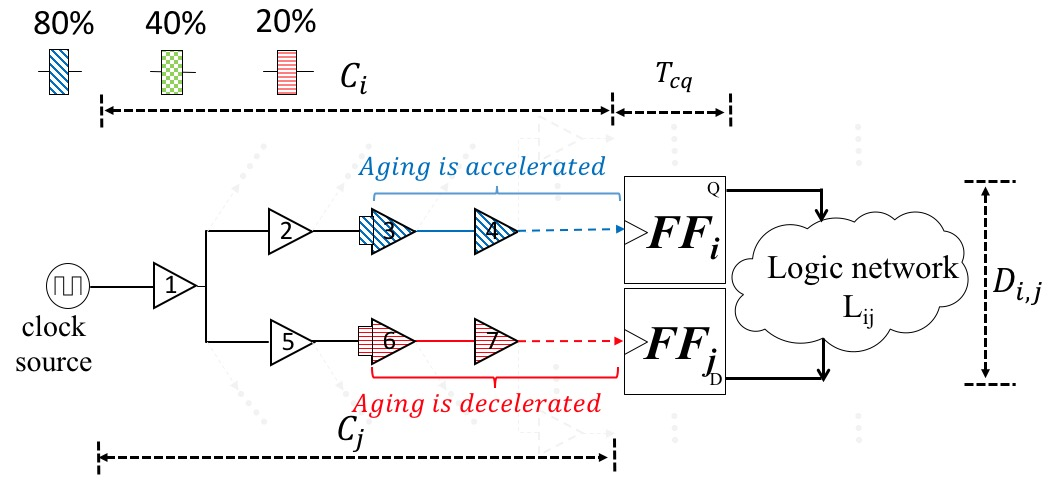
\includegraphics[width=0.9\columnwidth]{exp.png}
	\caption{Example of DCC insertion}
	\label{fig:mot}
\end{figure}

%--------------------------- DSN 2018 Version ----------------------------------------
\begin{comment}
\subsection{Duty-Cycle Converter (DCC)}
Duty cycle~\cite{wu2018maui} is the percentage of one period in which a signal is high (i.e., logic 1). We have known that the aging of logic gates highly depends on the stress time [8]. For a clock buffer on the clock tree, its stress time is proportional to the clock duty cycle. Therefore, by adjusting the clock duty cycle, we can manipulate the aging of clock buffers and then control the effective degradation of logic paths. Figure~\ref{fig:agr} shows the aging rates of clock buffers with different clock duty cycles.
The unit we use to change the clock duty cycle is duty-cycle converter (DCC). It converts the duty cycle of a clock signal to a smaller/larger one. Figure~\ref{fig:dcc} shows a DCC and the conversion of the clock duty cycle from 50\% to 80\%. It separates the source clock wave (black line) to a delayed wave (green line, may be inverted) and original wave. Then, those two waves are combined with the OR gate to obtain a new clock wave (red line) of 80\% duty cycle.
\subsection{DCCs against a Critical Path}
Once we insert a DCC into the clock tree, the downstream sub-tree of the DCC insertion point will receive a clock signal whose duty cycle is no longer 50\%. Consider the circuit in \ref{fig:mot}: we insert an 80\% DCC on the left clock path to accelerate its aging and a 20\% DCC on the right clock path to decelerate its aging. Over several years, the left clock latency will gain greater than the right one does. Therefore, setup-time violations are likely to occur on this critical path.
\end{comment}
%--------------------------- New Version ----------------------------------------
\subsection{Duty-Cycle Converter (DCC)}
Duty cycle is the percentage of one period in which a signal is high (i.e., logic 1). The aging of logic gates highly depends on the stress time~\cite{wang2010impact}. For a clock buffer on the clock tree, its stress time is proportional to the clock duty cycle. Therefore, by adjusting the clock duty cycle, we can manipulate the aging of clock buffers and then control the effective degradation of logic paths. The unit we use to change the clock duty cycle is duty-cycle converter (DCC)~\cite{wu2018maui}, which can converts the duty cycle of a clock signal to a smaller/larger one (e.g., $50\% \rightarrow 20\%$ or $50\% \rightarrow 80\%$). Once a DCC is inserted into the clock tree, the downstream sub-tree of the DCC insertion point will receive a clock signal whose duty cycle is no longer 50\%. This way, aging rate manipulation of downstream clock buffers can be achieved.
\subsection{DCCs against a Critical Path}
We use an illustrative example to explain our idea of shortening the lifespan of designs, by manipulating the aging rates of clock buffers. Consider the circuit in Figure~\ref{fig:mot}, where $FF_{i}$ and $FF_{j}$ are edge-triggered flip-flops and there exist seven buffers in the associated clock network. If the design needs work normally, the following setup-time constraint must be satisfied:
\begin{equation}
	\label{eq:setup}
	\fontsize{8}{9} \selectfont
	slack = (C_{j} + T_{c}) - (C_{i}  + T_{cq} + D_{ij} + T_{su}) > 0 
	%C_{i} + T_{cq} + D_{ij} + T_{su} < C_{j} + T_{c}
\end{equation}
where $C_{i}$ is the clock latency from clock source to $FF_{i}$, $C_{j}$ is the counterpart from clock source to $FF_{j}$, $T_{su}$ is setup time, $T_{c}$ is clock period, $T_{cq}$ is clock-to-output delay, and $D_{ij}$ is the largest path delay of logic network $L_{ij}$. The Equation~(\ref{eq:setup}) indicates the timing $slack$ must be greater than zero; otherwise, the transition through path $i$ does not have enough time to propagate to $FF_{j}$ within the current clock cycle, resulting in a timing error. For instance, the attacker inserts a 20\% DCC and an 80\% DCC at the inputs of buffers 6 and buffer 3, respectively. Over a period, $C_{i}$ will gain greater than $C_{j}$ does. This way, the timing $slack$ likely decreases to a negative value, such that setup-time violation occurs on this critical path, causing the failure of the designs.